\documentclass[11pt]{article}

\usepackage{amsmath,amssymb,amsfonts}
\usepackage{booktabs}
\usepackage{graphicx}
\usepackage{hyperref}
\usepackage{tikz}
\usepackage{xcolor}
\usepackage[margin=1in]{geometry}
\usepackage[numbers,square,sort&compress]{natbib}
\usepackage[affil-it]{authblk}
\usepackage{lineno}
\linenumbers

\renewcommand{\arraystretch}{1.3}
\setlength{\abovetopsep}{6pt}

\title{Construct Validity for Geometric Perturbation Scores:\\ When Does a Number License a Mechanistic Claim?}

\author{Elliot Tower}
\affil{Independent researcher \\ \texttt{elliot@elliottower.ai}}

\date{}

\begin{document}
\maketitle

\begin{abstract}
\textbf{Background:}
Geometric perturbation scores---such as direction instability, which
measures the angular consistency of perturbation signatures across
biological contexts---are used to rank drugs and genes by mechanism
conservation. These scores predict biological properties, but what
a given score \emph{licenses} as a mechanistic claim depends on
validity conditions that the raw number does not encode. We
propose a construct-validity framework (a ``validity ladder'') that
specifies which interpretive threats a score has survived, and test
whether these conditions matter empirically.

\textbf{Methods:}
We conducted pre-registered experiments across three perturbation
domains: 8{,}949 LINCS L1000 drug compounds, 1{,}676 Perturb-seq
CRISPRi gene knockdowns, and 25{,}254 JUMP-CP Cell Painting
morphological profiles. Five drug hypotheses and three genetic
hypotheses were tested with Holm--Bonferroni correction within each
domain family. Validity conditions included phenotype projection
onto genetic perturbation directions, transport-stable variance
correction with leave-one-out cross-validation, and essential-gene
confound correction on Grassmannian subspaces.

\textbf{Results:}
Domain-specific validity conditions preserved global rankings in all
three domains (LINCS: $\rho > 0.99$; Perturb-seq: $\rho = 0.91$;
JUMP-CP: $\rho = 0.99$) while upgrading inferential warrant at the
item level. Phenotype-projected scores correlated with on-target
genetic perturbation connectivity ($\rho = 0.38$, $p < 10^{-27}$)
while raw scores did not ($\rho = -0.04$). Transport-stable scores
outpredicted raw scores for held-out cell-line effects in all 66
valid leave-one-out folds (Wilcoxon $p = 8.2 \times 10^{-13}$;
mean $\Delta\rho = +1.10$, 95\% CI $[1.00, 1.19]$). Essential-gene
correction revealed that universal-essential knockdowns
\emph{diverge} rather than converge across cell types ($d = 0.60$,
$p_{\text{perm}} < 10^{-4}$), inverting the predicted confound.
Of 5 drug hypotheses, 2 survived multiplicity correction, 1 was
refuted, and 2 were informative nulls.

\textbf{Conclusions:}
Validity conditions do not change geometric perturbation scores;
they change what a practitioner can conclude from them. The
construct-validity framework tested here---applicable to any
geometric score that measures perturbation-response consistency
across contexts---provides a structured procedure for accumulating
interpretive evidence, separating scores that license mechanistic
claims from scores that merely rank.
\end{abstract}

\paragraph{Keywords:} construct validity, direction instability, geometric perturbation scores, LINCS L1000, Perturb-seq, Cell Painting, validity ladder, pre-registration, Fr\'{e}chet variance, Grassmannian geodesic

\section{Background}

Geometric perturbation scores---metrics that quantify how a biological
system's response to a perturbation varies across experimental
contexts---are used throughout computational biology to rank drugs, genes,
and compounds by mechanism conservation
\citep{lamb2006connectivity,subramanian2017next}. Direction instability,
one such score, measures the angular consistency of perturbation signatures
across cell lines: a drug whose transcriptomic response points in the same
direction regardless of cell type receives a low score, indicating conserved
mechanism \citep{tower2026drug}. Applied to 8{,}949 drugs in LINCS L1000,
direction instability produces biologically meaningful rankings: pan-HDAC
inhibitors achieve the lowest scores ($D = 0.14$--$0.19$), with a
selectivity gradient within the HDAC class (Figure~\ref{fig:hdac})
that tracks isoform specificity \citep{tower2026atlas}.

These rankings establish that the score captures genuine biological signal.
They leave open a different question: under what conditions does a
geometric perturbation score license a mechanistic \emph{claim}? A score
of $D = 0.55$ means signatures point in similar directions across cell
lines. It does not mean the drug acts through a specific pathway or that
the observation will replicate in a new context.

This gap between score and claim is a construct-validity problem
\citep{messick1995validity}. In Messick's framework, a score's meaning is
not inherent in the number; it depends on accumulating evidence from
multiple sources that the score measures what it purports to measure and
that interpretations drawn from it are warranted. The same principle
applies to geometric perturbation scores: a raw ranking may be
reproducible and biologically correlated, yet insufficient to license
mechanistic inference without additional validation evidence.

Three empirical threats illustrate this gap. First, a drug's low direction
instability could reflect a coherent off-target program rather than
on-target mechanism conservation---the raw score cannot distinguish the
two. Second, a drug with low direction instability in training data may
fail to predict a held-out cell line's response, because the raw metric
conflates genuine directional consistency with Fr\'echet variance from a
small number of contexts. Third, in genetic perturbation screens,
universal-essential knockdowns could inflate or deflate cross-cell-type
distances through a shared lethal-response subspace, contaminating
transport scores that appear mechanistically informative.

We formalize these threats through a validity ladder
(Figure~\ref{fig:ladder}): a sequence of seven conditions that
progressively strengthen what a geometric perturbation score licenses.
Each rung answers a specific threat to interpretation. The ladder is a
domain-specific instantiation of construct validation, analogous to the
Bradford Hill criteria for causal inference
\citep{freiesleben2025benchmarking}: satisfying more rungs does not change
the number, it changes what a practitioner is warranted in concluding
from it. The rung ordering reflects logical dependency---a reliable
measurement (Rung~2) is prerequisite for meaningful projection (Rung~5),
and localized signal (Rung~4) precedes phenotype alignment (Rung~5)---rather
than a strict hierarchy of evidence strength.

This paper tests whether validity conditions matter empirically across three
perturbation domains: 8{,}949 LINCS L1000 drug compounds
\citep{subramanian2017next}, 1{,}676 Perturb-seq genetic knockdowns
\citep{replogle2022mapping}, and 25{,}254 JUMP-CP Cell Painting morphological
profiles \citep{chandrasekaran2023jump}. Direction instability serves as
the case study, but the construct-validity procedure---define threats,
specify corrections, pre-register predictions, test whether corrections
reorganize rankings or preserve them---applies to any geometric score
measuring perturbation-response consistency across contexts. We report
honest nulls alongside confirmations, because the pattern of where
validity conditions matter---and where they do not---is itself the finding.

\section{Definitions and notation}

\subsection{Direction instability}

For a drug tested in $K$ cell lines, let $\mathbf{s}_1, \ldots,
\mathbf{s}_K \in \mathbb{R}^{978}$ denote its consensus signature vectors.
Define unit-normalized signatures $\hat{\mathbf{s}}_i = \mathbf{s}_i /
\|\mathbf{s}_i\|_2$. Direction instability is:
\begin{equation}
  D = 1 - \frac{2}{K(K-1)} \sum_{i < j}
    \hat{\mathbf{s}}_i^\top \hat{\mathbf{s}}_j
  \label{eq:direction_instability}
\end{equation}
$D = 0$ when all signatures are collinear. $D = 1$ when orthogonal on average.
Cosine normalization renders direction instability invariant to perturbation
magnitude (Figure~\ref{fig:dag}): variance-based and estimation-based metrics
conflate perturbation strength with biological signal, but direction
instability measures only direction \citep{tower2026drug}.

\begin{figure}[t]
\centering
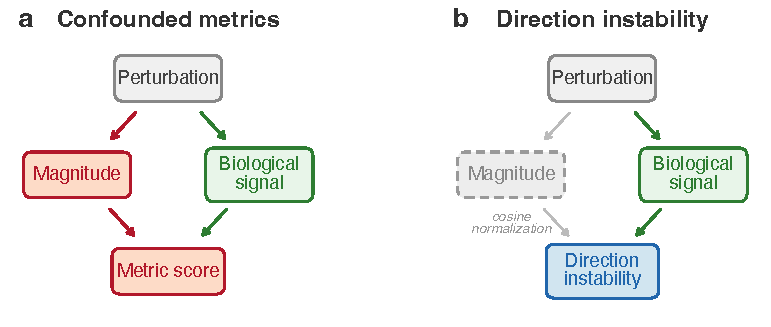
\includegraphics[width=\linewidth]{figures/fig1_dag_v3.pdf}
\caption{%
\textbf{Direction instability is invariant to perturbation magnitude.}
\textbf{(a)}~Confounded metrics (variance, subspace size) inherit effect
magnitude through a shared path, producing spurious associations between
perturbation strength and metric value.
\textbf{(b)}~Direction instability operates after cosine normalization,
which renders the metric invariant to perturbation magnitude. The observed
association between group variable and metric reflects biological signal only.
This invariance is necessary but not sufficient: direction instability still
requires validity conditions to distinguish on-target from off-target
consistency (Rung~5) and genuine transport from sampling noise (Rung~6).}
\label{fig:dag}
\end{figure}

\subsection{Grassmannian geodesic distance in Perturb-seq}

Direction instability generalizes from vectors to subspaces. For a gene
knocked down in two cell types, let $U_1, U_2 \in \text{Gr}(k, d)$ denote
the top-$k$ PCA subspaces of the perturbation response in each cell type
($k$ = subspace dimension, $d$ = ambient dimension).
The Grassmannian geodesic distance $\delta(U_1, U_2) =
\|\boldsymbol{\theta}\|_2$, where $\boldsymbol{\theta}$ are the principal
angles between the subspaces, measures how much the perturbation response
\emph{rotates} across cell types. With $K = 2$ contexts, this reduces to a
single pairwise comparison---a weaker geometric estimand than the
$K \geq 5$ angular-consistency computation used in LINCS and JUMP-CP,
as it carries no Fr\'{e}chet variance or holonomy information. We interpret
the Perturb-seq results accordingly.

\subsection{Direction instability in Cell Painting morphological profiles}

Cell Painting \citep{chandrasekaran2023jump} measures 3{,}180 morphological
features per well across five fluorescent channels. JUMP-CP
profiles 116{,}000 compounds across 10 imaging sources. Direction
instability applies directly: each compound's morphological signature in a
given source is a vector in $\mathbb{R}^{3180}$, and $D$ measures angular
consistency across sources. A subset of 743 features---cell area, compactness,
eccentricity, DNA/Mito intensity, granularity, and radial
distribution---reflect general cell health rather than compound-specific
morphological effects. The cell-health correction removes these features
before recomputing direction instability.

\subsection{The validity problem}

Consider two drugs with identical direction instability, $D = 0.55$:

\begin{itemize}
  \item \textbf{Drug A} is a pan-HDAC inhibitor. Its conserved direction
    aligns with its target gene's knockdown signature---phenotype-projected
    bracket is high. The consistency comes from on-target chromatin
    remodeling.
  \item \textbf{Drug B} is an off-target consistent compound. Its conserved
    direction does \emph{not} align with its annotated target's knockdown
    signature---phenotype-projected bracket is near zero. The consistency
    comes from an off-target program shared across cell types.
\end{itemize}

Both achieve $D = 0.55$. Both pass the raw metric equally. Phenotype
projection (Rung~5 of the validity ladder) distinguishes them: Drug~A's
consistency is mechanistically on-target; Drug~B's is not. The distinction
matters for downstream decisions: Drug~A is a strong candidate for
mechanism-based repurposing; Drug~B requires additional investigation to
identify what program drives its consistency before any mechanistic claim
is warranted.

\subsection{The validity ladder}

The validity ladder is a domain-specific instantiation of Messick's
construct-validation framework \citep{messick1995validity}, adapted for
geometric perturbation scores. We define seven rungs
(Figure~\ref{fig:ladder}), ordered by logical dependency rather than by
evidence strength:

\begin{enumerate}
  \item \textbf{Process view declared.} What constitutes a ``context''?
  \item \textbf{Reliable vector field.} Adequate signal-to-noise for
    direction to be meaningful.
  \item \textbf{Perturbation estimable.} Effect isolated from background.
  \item \textbf{Localized to biology.} Instability concentrates in
    pathway-relevant genes.
  \item \textbf{Phenotype-aligned.} Conservation direction matches a
    known target pathway.
  \item \textbf{Transports across contexts.} Score replicates in held-out
    contexts (low Fr\'echet variance).
  \item \textbf{Predicts holdout.} Metric predicts an external outcome
    in new data.
\end{enumerate}

Rungs 1--3 are satisfied by design in our datasets and are not tested
further. Rungs 4--6 are the validity conditions we test empirically.
Rung~7 (holdout prediction in a genuinely new dataset) is not tested:
Experiment~5's leave-one-cell-line-out cross-validation tests Rung~6
(transport within LINCS), not generalization to an independent dataset.

\begin{figure}[t]
\centering
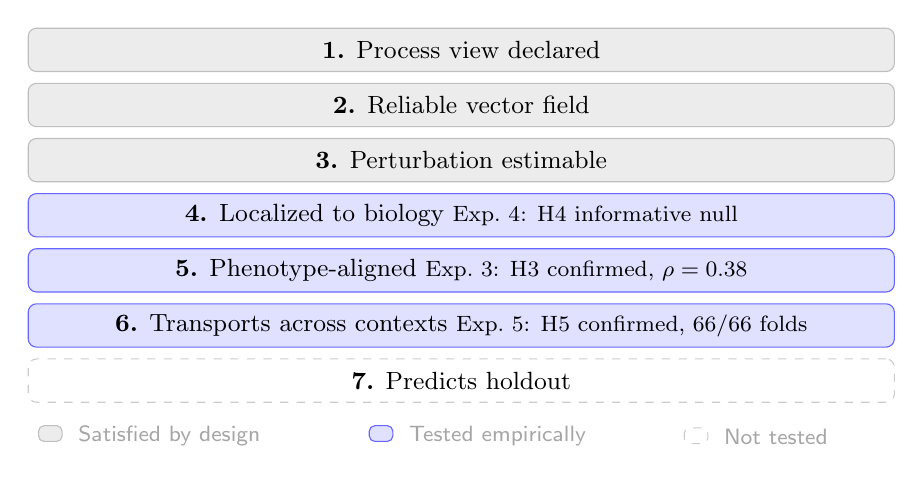
\begin{tikzpicture}[
  rung/.style={draw, rounded corners=3pt, minimum width=11cm, minimum height=0.55cm, font=\small},
  satisfied/.style={rung, fill=gray!15, draw=gray!50},
  tested/.style={rung, fill=blue!12, draw=blue!60},
  untested/.style={rung, fill=white, draw=gray!40, dashed},
  label/.style={font=\footnotesize\sffamily, text=gray!70},
]
\node[untested]  at (0, 0.0) {\textbf{7.} Predicts holdout};
\node[tested]    at (0, 0.7) {\textbf{6.} Transports across contexts \hfill \textnormal{\footnotesize Exp.~5: H5 confirmed, 66/66 folds}};
\node[tested]    at (0, 1.4) {\textbf{5.} Phenotype-aligned \hfill \textnormal{\footnotesize Exp.~3: H3 confirmed, $\rho = 0.38$}};
\node[tested]    at (0, 2.1) {\textbf{4.} Localized to biology \hfill \textnormal{\footnotesize Exp.~4: H4 informative null}};
\node[satisfied] at (0, 2.8) {\textbf{3.} Perturbation estimable};
\node[satisfied] at (0, 3.5) {\textbf{2.} Reliable vector field};
\node[satisfied] at (0, 4.2) {\textbf{1.} Process view declared};
% Legend
\node[label, anchor=west] at (-5.5, -0.7) {%
  \tikz\draw[fill=gray!15, draw=gray!50, rounded corners=2pt] (0,0) rectangle (0.3,0.2);
  ~Satisfied by design};
\node[label, anchor=west] at (-1.3, -0.7) {%
  \tikz\draw[fill=blue!12, draw=blue!60, rounded corners=2pt] (0,0) rectangle (0.3,0.2);
  ~Tested empirically};
\node[label, anchor=west] at (2.7, -0.7) {%
  \tikz\draw[fill=white, draw=gray!40, dashed, rounded corners=2pt] (0,0) rectangle (0.3,0.2);
  ~Not tested};
\end{tikzpicture}
\caption{%
\textbf{The validity ladder.}
Seven rungs progress from measurement prerequisites (1--3)
through empirically tested validity conditions (4--6) to external
prediction (7). Each rung eliminates a specific interpretive threat.
Rungs~4--6 are tested across three domains (LINCS L1000, Perturb-seq,
JUMP-CP); result summaries are shown at right. Satisfying additional
rungs does not change the direction-instability score---it upgrades the
inferential warrant attached to it.}
\label{fig:ladder}
\end{figure}

\begin{figure}[t]
\centering
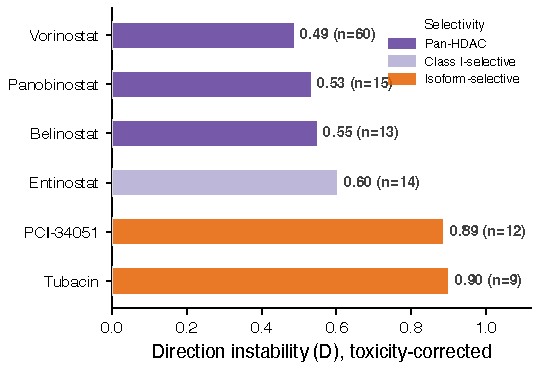
\includegraphics[width=0.85\linewidth]{figures/fig5_hdac.pdf}
\caption{%
\textbf{HDAC selectivity gradient: calibration standard for direction
instability.}
Pan-HDAC inhibitors (panobinostat, vorinostat, belinostat) achieve the
lowest direction instability ($D = 0.14$--$0.19$); Class~I-selective
entinostat is intermediate ($D = 0.27$); isoform-selective HDAC6 and HDAC8
inhibitors (tubacin, PCI-34051) have the highest instability within the
class ($D = 0.32$--$0.45$). This gradient, reproduced from
\citet{tower2026drug}, provides a fine-grained rank ordering within the
HDAC class: Spearman $\rho = 0.83$ between direction instability and
selectivity rank across these 6 compounds after toxicity-gene correction.
The HP1 ``doesn't bite'' threshold ($\rho \geq 0.83$) was calibrated to
this value.}
\label{fig:hdac}
\end{figure}

\section{Related work}

\paragraph{Construct validity in measurement.}
Messick's unified validity framework \citep{messick1995validity} established
that a score's meaning depends on accumulating evidence across multiple
sources---content, substantive, structural, generalizability, external,
and consequential. Our validity ladder instantiates this framework for
geometric perturbation scores: Rungs~1--3 address content and structural
validity, Rungs~4--5 address substantive and external validity, and
Rung~6 addresses generalizability. Recent construct-validity
frameworks for computational scores \citep{freiesleben2025benchmarking,
watson2025measuring} and the SBB principles for perturbation-prediction
models \citep{sbb2026principles} share this orientation.

\paragraph{Perturbation biology.}
CERES \citep{meyers2017ceres} corrects copy-number artifacts in CRISPR
screens; integrated Broad--Sanger analyses \citep{pacini2021integrated}
document cross-study divergence. These corrections operate on
dependency-score magnitudes; our contribution is orthogonal, correcting
subspace geometry and showing that rank-preserving corrections carry
inferential value. The Connectivity Map framework
\citep{subramanian2017next,lamb2006connectivity} and subsequent metric
evaluations \citep{li2020comprehensive} establish the
transcriptomic-similarity paradigm that direction instability extends.
LEMUR \citep{ahlmanneltze2025lemur} performs multivariate regression on
Grassmann manifolds for multi-condition Perturb-seq; our Experiment~7 uses
a simpler Grassmannian geodesic distance.

\section{Methods}

\subsection{Data}

Perturbation signatures were drawn from LINCS L1000 Phase~I (GEO accession
GSE92742; $\sim$1.3 million profiles across $\sim$50 cell lines),
using Level~5 replicate-collapsed z-scores across 978 landmark genes
\citep{subramanian2017next}. We retained 8{,}949 small-molecule
perturbagens tested in $\geq5$ cell lines.

Perturb-seq data derive from \citet{replogle2022mapping}: genome-scale
CRISPRi knockdowns in K562 and RPE1 cells. We extracted 1{,}676 genes
with $\geq$30 perturbed cells in both cell types, computed per-gene
expression responses over 2{,}073 highly variable genes, and fitted
$k = 5$ PCA subspaces per gene per cell type (of these, 1{,}567 have
matching DepMap Chronos labels for HP3; all 1{,}676 are used for HP1).
Both screens target DepMap-essential genes; 85\% of RPE1 targets overlap
with K562 targets. Essentiality labels derive from DepMap Chronos scores
\citep{dempster2021chronos}: 855 genes with Chronos $< -0.5$ in both
K562 and RPE1 were classified as universal-essential; the remaining 712
are sub-threshold and serve as the comparison group. A label-permutation
null (10{,}000 permutations) tested whether the observed group difference
exceeds background K562/RPE1 divergence.

JUMP-CP Cell Painting profiles derive from the Cell Painting Gallery
\citep{chandrasekaran2023jump}: 25{,}254 compounds tested in $\geq$5
imaging sources after filtering (78\% attrition from the 116{,}750
total; the majority of compounds appear in fewer than 5 sources,
making direction instability---which requires multiple
contexts---undefined for them). Cell-health features (743 features matching Area,
Compactness, Eccentricity, DNA/Mito Intensity, Granularity, Radial
Distribution, and Texture Entropy) were identified by substring matching
on CellProfiler feature names; corrected direction instability was computed
on the remaining 2{,}437 features.

All scoring functions and drug lists were committed before any real LINCS
signatures were analyzed (initial freeze: commit \texttt{8d74bd0}).
Perturb-seq hypotheses and extended drug hypotheses (H5-full,
H3-CRISPRi) were pre-registered before the correction analysis
(commit \texttt{f3c88ed}, tag \texttt{prereg-extended-psb}, timestamped
2026-07-08 11:56:58 UTC, preceding experiment execution at
${\sim}$12:00--12:15 UTC). The repository was public at the time of both
freezes.\footnote{Code, pre-registration, deviation log, and all
experimental scripts:
\url{https://github.com/elliottower/direction-instability-drug-validity}.
LINCS data: GEO GSE92742; Perturb-seq: \citet{replogle2022mapping};
JUMP-CP: \citet{chandrasekaran2023jump}; DepMap: \citet{dempster2021chronos}.}

We treat the five LINCS hypotheses (H1--H5) as one test family and the
three Perturb-seq hypotheses (HP1--HP3) as a second, because the two
domains use different data sources, perturbation types, and geometric
estimands (vector cosines vs.\ Grassmannian geodesics), making a joint
family overly conservative. After Holm--Bonferroni
correction within the drug family, H3 ($p < 10^{-27}$) and H5
($p_{\text{Wilcoxon}} = 8.2 \times 10^{-13}$; also
$p_{\text{perm}} < 10^{-3}$ on the preliminary 5-fold analysis) survive
at $\alpha = 0.05$; H2 ($p = 0.28$) and H4 (gap $= 0.018$) do not;
H1's criterion-pass is an artifact.
Within Perturb-seq, HP3 ($p_{\text{perm}} < 10^{-4}$) survives.

\subsection{Phenotype-projected bracket (Experiment 3)}

For each drug with an annotated target gene (Drug Repurposing Hub,
1{,}551 drugs), the ``on-target direction'' is the consensus shRNA
knockdown signature of that target gene in LINCS L1000 (4{,}369 genes
eligible, $\geq$3 hairpins each, consensus averaged across 20 cell lines).
Phenotype-projected bracket projects the instability vector onto this
on-target direction. On-target enrichment is quantified by cosine squared
between each drug's mean signature and its target gene's shRNA consensus.

shRNA signatures have well-documented off-target effects, which add noise
to the on-target direction. The shRNA consensus averages across
${\sim}20$ cell lines, producing a cell-type-agnostic on-target
direction at the cost of off-target contamination. A convergent-validity
check using CRISPRi signatures (single cell type, cleaner
loss-of-function but cell-type-specific) is reported in the Results.

The pre-registered prediction (H3) required Spearman $|\rho| > 0.3$ between
phenotype-projected bracket and on-target enrichment, and $|\rho| < 0.15$
for raw bracket versus the same enrichment.

\subsection{Transport-stable bracket (Experiment 5)}

Transport-stable bracket penalizes raw direction instability by Fr\'{e}chet
variance across contexts:
\begin{equation}
  \text{TS} = D - \lambda \cdot \text{Var}_{\text{Fr\'echet}}
  \label{eq:ts}
\end{equation}
where $\text{Var}_{\text{Fr\'echet}} = \frac{1}{K}\sum_i
\arccos^2(\hat{\mathbf{s}}_i^\top \bar{\mathbf{s}})$ and
$\bar{\mathbf{s}}$ is the Fr\'echet mean direction. The subtraction is a
heuristic combination: the alternative (a ratio) would be undefined when
$\text{Var}_{\text{Fr\'echet}} = 0$ and would amplify noise for highly
consistent drugs. The penalty weight $\lambda$ was fixed at the value from
\citet{tower2026drug} and was not optimized for this evaluation.

We evaluate via leave-one-cell-line-out cross-validation over all cell
lines with $\geq 20$ eligible drugs after excluding the held-out cell line
(66 valid folds out of 71 total; 5 excluded for insufficient drug count).
A preliminary 5-fold analysis using alphabetically-selected cell lines
(A375, A549, A673, AGS, ASC) established the rare/common regime distinction
with permutation nulls; the full leave-one-out extends this to all cell
lines and adds Wilcoxon signed-rank as a co-primary criterion.

The pre-registered prediction (H5) required TS to outpredict raw bracket
in $\geq 80\%$ of valid folds (co-primary~1), with Wilcoxon signed-rank on
per-fold $\Delta\rho$ rejecting $H_0$: median $\leq 0$ at $\alpha = 0.05$
(co-primary~2).

\subsection{Essential-gene correction on Perturb-seq (Experiment 7)}

We computed the Fr\'echet mean subspace of the 855 essential-gene
perturbation responses (separately in K562 and RPE1) via iterative
projection on Gr$(5, 2073)$ (100 iterations, convergence to
$\Delta < 10^{-6}$ in Grassmannian distance; the result is insensitive
to initialization because the essential-gene subspaces cluster tightly).
We then projected this essential-response subspace out of each gene's
response subspace, re-orthogonalized, and recomputed geodesic distances.

Two pre-registered predictions were tested.
HP1 required Spearman $\rho$ between raw and corrected distances below
0.70 (``bites'') or $\geq 0.83$ (``doesn't bite'').
HP3 predicted that universal-essential knockdowns produce higher geodesic
distances than non-essential knockdowns (Cohen's $d > 0$).

\subsection{Cell-health correction on JUMP-CP (Experiment 8)}

The 743 cell-health features constitute 23\% of the 3{,}180-feature
space---proportionally six times larger than the LINCS toxicity gene set
(41/978, 4\%) and the largest feature removal in this study. If cell-health
variance dominates cross-source consistency, this correction should
reorganize the ranking more substantially than the drug or genetic
corrections. This makes Experiment~8 the strongest test of the thesis:
if corrections don't bite even when the removed feature set is
proportionally large, the ranking is robust.

The pre-registered prediction used the same threshold: Spearman $\rho$
between raw and corrected direction instability below 0.70 (``bites'')
or $\geq 0.83$ (``doesn't bite'').

\subsection{Supplementary experiments}

Three additional drug-domain experiments are reported in the Additional
files (available in the code repository). \textbf{Experiment~1}
(H1, toxicity correction) tests whether cytotoxic drugs masquerade as
mechanism-conserving. \textbf{Experiment~2} (H2, broad-mechanism drugs)
tests whether broad-target therapeutics fall below the population median.
\textbf{Experiment~4} (H4, localization score) tests whether gene-set
restriction improves MOA prediction. HP2 (GO pathway prediction from
corrected Perturb-seq distances) is also in the Additional files.

\section{Results}

\subsection{Pre-registered scorecard}

Table~\ref{tab:scorecard} summarizes all pre-registered hypotheses.
Two of five drug hypotheses survive Holm--Bonferroni correction (H3, H5);
H2 meets its pre-registered criterion but does not survive multiplicity
correction; H1 is refuted with an artifact criterion-pass; H4 is an
informative null.
In the Perturb-seq domain, HP3 is confirmed; HP1 shows the correction
``doesn't bite'' at the population level; HP2 is a null. Experiment~8
(JUMP-CP) shows the correction ``doesn't bite.''

\begin{table}[t]
\centering
\caption{Pre-registered scorecard. Hypotheses are grouped by domain.
``Holm'' indicates survival after Holm--Bonferroni correction within
the drug family ($\alpha = 0.05$). Experiment references are to the
full methods in the body (Exp.~3, 5, 7, 8) or Additional files
(Exp.~1, 2, 4). Result details for starred entries appear in Section~5.6.}
\label{tab:scorecard}
\small
\begin{tabular}{llllc}
\toprule
 & Prediction & Result & Outcome & Holm \\
\midrule
H1$^\star$ & Toxicity reclassifies & $\Delta < 0.01$ & Refuted & --- \\
H2$^\star$ & Broad drugs below median & 7/10 below & Confirmed & No \\
H3 & $|\rho_{\text{proj}}| > 0.3$ & $\rho = 0.376$ & Confirmed & Yes \\
H4$^\star$ & AUROC gap $> 0.05$ & Gap $= 0.018$ & Null & No \\
H5 & TS wins $\geq$80\% folds & 66/66 folds, $p_W = 8.2 \times 10^{-13}$ & Confirmed & Yes \\
\midrule
HP1 & Correction bites ($\rho < 0.70$) & $\rho = 0.91$ & Doesn't bite & --- \\
HP2$^\star$ & GO prediction improves & $\Delta\rho = -0.02$ & Doesn't bite & --- \\
HP3 & Essential $d > 0$ & $d = 0.60$ & Confirmed & Yes \\
\midrule
Exp.~8 & Health correction bites & $\rho = 0.987$ & Doesn't bite & --- \\
\bottomrule
\end{tabular}
\end{table}

\subsection{Experiment 3: Phenotype-projected bracket separates on-target from off-target instability}

Among 795 drugs with annotated targets and matched shRNA consensus signatures,
phenotype-projected bracket correlates with on-target enrichment at Spearman
$\rho = 0.376$ ($p = 4.8 \times 10^{-28}$). Raw bracket shows no correlation
($\rho = -0.043$, $p = 0.22$). Both pre-registered criteria are satisfied.

H3 confirms Rung~5 of the validity ladder. Raw direction instability
measures whether a drug's signatures point in consistent directions, but
this consistency could arise from any coherent program. Projecting onto the
genetic perturbation direction of the annotated target isolates the
mechanistically relevant component. The near-zero raw correlation shows
that global instability carries no on-target information; the strong
projected correlation shows that the on-target projection recovers it.

The gene-set construction avoids researcher degrees of freedom: the shRNA
consensus is an empirical object from the same LINCS platform,
requiring no pathway database selection. H3 and H4 share this shRNA
dependency (documented in DEVIATION\_LOG.md entry~3) and are not
independent tests. The phenotype-projected bracket is applicable only
to drugs with target annotations---1{,}551 of 8{,}949 (17\%). For the
remaining 82\% of drugs with unknown targets, the validity ladder
provides other rungs (transport stability, localization) that do not
require target annotations.

As a pre-registered convergent-validity check, we recomputed
phenotype-projected bracket using CRISPRi loss-of-function signatures
\citep{replogle2022mapping} as the on-target
direction. The projected-bracket correlation with on-target enrichment
did not reach significance (Spearman $\rho = -0.12$, $p = 0.16$,
$n = 131$), corresponding to pre-registered outcome~(c). On the
114-drug matched subset (drugs with both ground truths), shRNA
projection yields $\rho = 0.42$ while CRISPRi projection yields
$\rho = -0.14$, confirming that the ground-truth source---not the
drug set---drives the difference.

The pre-registered secondary criterion points to the likely cause: raw
bracket correlated positively with CRISPRi enrichment
($\rho = +0.27$, $p = 0.002$) while projected bracket did not---the
reverse of the shRNA pattern. This reversal is consistent with the
pre-registered K562-only confound: CRISPRi signatures derive from a
single hematopoietic cell type, so the CRISPRi ``on-target direction''
captures cell-type-specific effects rather than cross-context
mechanism---a confound that multi-cell-line shRNA consensus avoids by
averaging across ${\sim}20$ cell lines. One plausible explanation for
the positive raw-bracket/CRISPRi correlation, which we did not test
directly, is that K562 expresses many drug targets at high levels,
producing spurious alignment between raw instability and K562-specific
signatures.

CRISPRi does not provide independent convergent validity for H3. The
shRNA-based result stands on its original evidence rather than being
reinforced.

\subsection{Experiment 5: Transport-stable bracket outpredicts raw bracket in held-out cell lines}

Transport-stable bracket outpredicts raw bracket in all 66 valid
leave-one-out folds. Both co-primary criteria are satisfied:
TS wins 66/66 folds (100\%, criterion $\geq 80\%$) and Wilcoxon
signed-rank on per-fold $\Delta\rho$ yields $p = 8.2 \times 10^{-13}$
(criterion $p < 0.05$).

Across 66 folds, mean raw $\rho = -0.60$ (anti-predictive in every
fold; range $[-0.78, -0.22]$) while mean TS $\rho = +0.50$ (positively
predictive). Mean $\Delta\rho = +1.10$ (95\% bootstrap CI
$[1.00, 1.19]$; all 66 values positive, range $[0.17, 1.57]$). Five
cell lines were excluded for having $< 20$ eligible drugs.
Figure~\ref{fig:delta_rho} shows the $\Delta\rho$ distribution and the
frequency gradient; Table~\ref{tab:transport} shows representative folds
illustrating the rare/common regime distinction.

\begin{figure}[t]
\centering
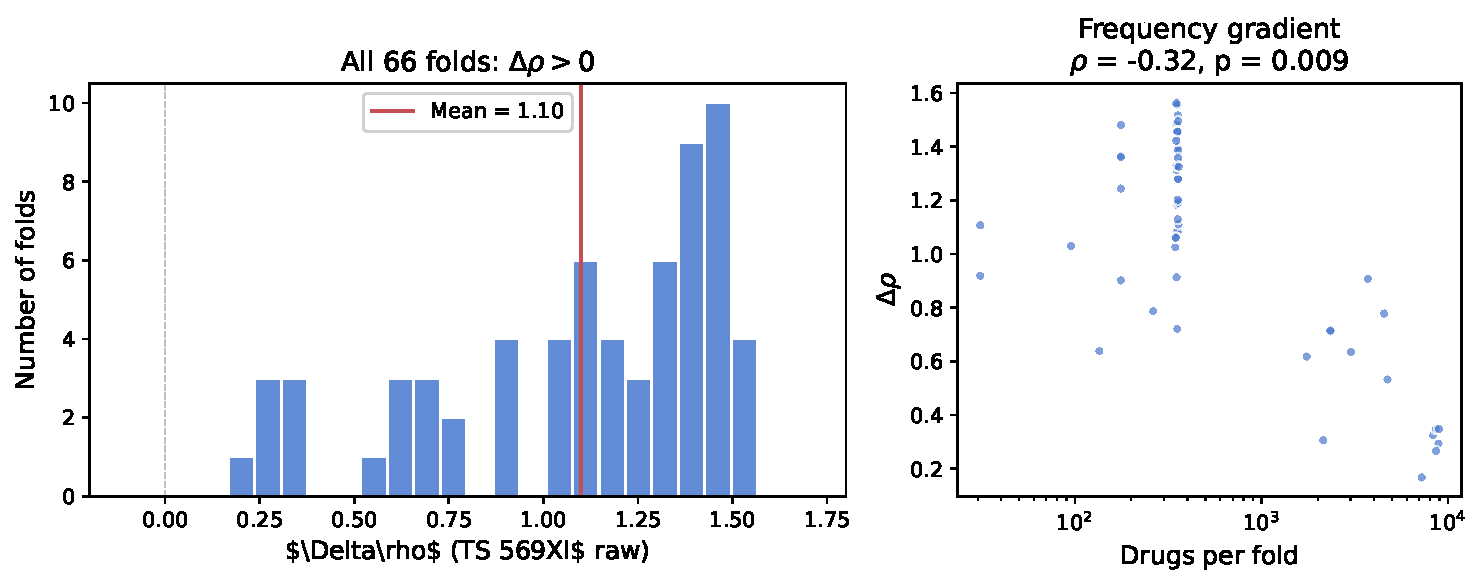
\includegraphics[width=\linewidth]{figures/fig_h5_full_delta_rho.pdf}
\caption{%
\textbf{Full 66-fold leave-one-out: TS advantage is universal.}
\textbf{Left:}~Distribution of per-fold $\Delta\rho$ (TS $-$ raw Spearman
correlation with held-out cosine). All 66 values are positive; the mean
(red line) is $+1.10$. \textbf{Right:}~Rarer cell lines (fewer drugs per
fold) show larger TS advantages (Spearman $\rho = -0.32$, $p = 0.009$),
confirming that the rare/common regime distinction from the preliminary
5-fold analysis generalizes across all cell lines.}
\label{fig:delta_rho}
\end{figure}

\begin{table}[t]
\centering
\caption{Leave-one-cell-line-out cross-validation (selected folds from
the full 66-fold analysis). Transport-stable (TS) bracket outpredicts
raw bracket in all folds. In common folds (8{,}000+ drugs), both metrics
are anti-predictive but TS is less so. In rarer folds, TS reverses the
sign entirely. Full 66-fold results: mean $\Delta\rho = +1.10$,
Wilcoxon $p = 8.2 \times 10^{-13}$.}
\label{tab:transport}
\small
\begin{tabular}{lrrrl}
\toprule
Held-out cell & $N_{\text{drugs}}$ & $\rho_{\text{raw}}$ & $\rho_{\text{TS}}$ & Winner \\
\midrule
A375 & 8{,}328 & $-$0.480 & $-$0.155 & TS \\
A549 & 8{,}888 & $-$0.494 & $-$0.201 & TS \\
A673 & 357 & $-$0.725 & $+$0.725 & TS \\
AGS & 356 & $-$0.712 & $+$0.714 & TS \\
ASC & 2{,}345 & $-$0.365 & $+$0.346 & TS \\
\bottomrule
\end{tabular}
\end{table}

In rarer folds (such as A673, AGS, ASC), raw bracket is strongly
anti-predictive ($\rho = -0.37$ to $-0.73$): drugs with high raw
instability in training produce held-out signatures that point
\emph{away} from the training consensus. Transport-stable bracket
reverses this, becoming positively predictive ($\rho = +0.35$ to
$+0.73$). The reversal occurs because removing a single rare cell
line substantially changes the consensus direction; drugs whose
training instability was driven by that cell line are precisely those
that TS downweights via the Fr\'{e}chet penalty. This pattern holds
across all 66 folds: the frequency-improvement correlation (Spearman
$\rho = -0.32$, $p = 0.009$) confirms that rarer cell lines show
larger TS advantages.

In common folds (8{,}000+ drugs), both metrics remain
anti-predictive. TS improves over raw ($\rho = -0.155$ vs.\ $-0.48$ for
A375; $-0.201$ vs.\ $-0.49$ for A549), but both correlations stay
negative. TS ``wins'' in these folds by losing less badly, not by becoming
positively predictive. The consensus direction is stable when computed from
many cell lines, leaving less room for the Fr\'{e}chet penalty to
improve prediction.

Raw direction instability is anti-predictive because it conflates two
sources of angular consistency: genuine mechanism conservation (signal)
and the geometric tightness of the consensus direction around a small
number of contexts (noise). Drugs with low raw DI in training tend to
have tight consensus directions that are sensitive to removing any single
cell line---precisely the drugs that fail to predict held-out effects.
This is a failure of the raw estimator when applied to leave-one-out
prediction without variance correction, not a failure of direction
instability as a concept.

Before conducting the full 66-fold leave-one-out, we tested whether the
TS advantage could be algebraic using a variance-preserving permutation
null on the preliminary 5-fold analysis. Held-out
\emph{signatures} are shuffled across drugs while training data
(raw DI, Fr\'echet variance, TS, consensus vector) remain fixed,
and held-out cosines are recomputed against each drug's original
consensus. Under this null (1{,}000 permutations),
TS wins only 0.1 of 5 folds on average with mean $\Delta\rho = -0.12$
(raw DI \emph{outpredicts} TS when drug-specific signal is broken).
The observed advantage falls entirely outside the null distribution
($p_{\text{perm}} < 10^{-3}$). The full 66-fold Wilcoxon test
($p = 8.2 \times 10^{-13}$) provides independent confirmation that the
advantage is drug-specific.

\subsection{Experiment 7: Essential-gene correction preserves ranking
but reveals confound-dominated machinery}

Universal-essential knockdowns have \emph{higher} Grassmannian geodesic
distances than non-essential knockdowns (mean 2.80 vs.\ 2.67, Cohen's $d =
+0.60$, Mann--Whitney $p < 10^{-33}$; $n = 1{,}567$ genes with both
geodesic distances and DepMap labels, of which 855 universal-essential and
712 sub-threshold). Cohen's $d = 0.60$ is a medium effect---the
distributions overlap substantially, and individual genes span the full
range in both groups. The finding is that the \emph{group means} differ
in the opposite direction from the predicted confound, not that essentiality
status determines geodesic distance.

Essential genes do not produce a shared response across cell types; they
\emph{diverge}---the same gene's lethal disruption manifests through
different transcriptomic programs in K562 and RPE1
(Figure~\ref{fig:cross_domain}). This is consistent with cell-line-specific
essentiality effects documented in CERES \citep{meyers2017ceres} and
integrated Broad--Sanger analyses \citep{pacini2021integrated}: the
functional consequences of losing a core-machinery gene depend on
the cell's lineage and metabolic context.

A label-permutation null (shuffling essential/non-essential labels across
the 1{,}567 genes, 10{,}000 permutations) confirms that this divergence
exceeds background K562/RPE1 divergence: the observed difference (0.123)
falls outside the null 95\% interval $[-0.021, 0.022]$,
$p_{\text{perm}} < 10^{-4}$. The null preserves the geodesic-distance
distribution while breaking only the label assignment, so the ${\sim}6\times$
exceedance of the null half-width rules out the library-overlap confound
(85\% target overlap between screens).

Spearman $\rho$ between raw and corrected geodesic distances is 0.91
($p < 10^{-100}$). The global ranking is preserved.

The correction's value is at the item level: individual genes shift
hundreds of rank positions. The top 100 rank-shifters are enriched for
spliceosomal complex assembly (Fisher's exact OR $= 8.9$,
$p = 1.3 \times 10^{-7}$) and proteasomal catabolic processes
(OR $= 4.1$, $p = 6.7 \times 10^{-5}$). Proteasome subunits
(\emph{PSMA3}, \emph{PSMB6}, \emph{PSMC4}) shift 750--900 positions;
spliceosome components (\emph{SF3B1}, \emph{SNRPG}, \emph{DDX23}) shift
660--820 positions. These core-machinery complexes are the genes whose
cross-cell-type geometry is most dominated by the shared essential-response
axis. The correction provides a concrete action: flag these genes before
interpreting their transport scores.

\subsection{Experiment 8: Cell-health correction has negligible
effect in JUMP-CP}

Among 25{,}254 compounds, corrected direction instability tracks raw
at Spearman $\rho = 0.987$ ($p < 10^{-100}$). By the pre-registered
criterion, this ``doesn't bite''---the strongest result for ranking
robustness across all three domains.

The 743 health features constitute 23\% of the 3{,}180-feature
space---proportionally six times larger than the drug toxicity gene set
(41/978, 4\%)---yet produce \emph{less} ranking impact ($\rho = 0.987$
vs.\ $\rho > 0.99$ for LINCS). That a proportionally larger feature
removal barely moves the ranking is stronger evidence for the thesis than
the drug case: cell-health features carry less of the cross-source
variance in morphological signatures than stress genes carry in
transcriptomic signatures. The 78\% attrition from the full JUMP-CP
dataset (116{,}750 to 25{,}254 compounds) means the retained set is
biased toward well-replicated compounds; the result may not generalize
to sparsely-profiled compounds.

One explanation for the negligible effect: in morphological space,
``health'' and ``mechanism'' features are less separable than in
transcriptomic space. A drug that alters cell shape changes both
health-associated features (area, compactness) and mechanism-specific
features (texture, radial distribution) simultaneously, because
morphological effects are inherently coupled. In 978-gene transcriptomic
space, stress-response genes and pathway-specific genes are more
separable, which is why the LINCS toxicity correction has a larger
(though still small) effect.

Despite near-perfect global correlation, individual compounds shift up
to 7{,}155 rank positions, identifying those whose apparent morphological
consistency is health-feature-dominated. The cell-health feature
definition (substring matching on CellProfiler names) is a limitation:
a partition based on correlation with viability assays would be more
principled and could yield different correction magnitudes.

\subsection{Summary of supplementary experiments}

Full methods, tables, and discussion appear in the Additional files.

\textbf{H1 (toxicity correction).} Among 13 cytotoxic drugs, most are already high-instability ($D > 0.87$
for 9 of 13); toxicity correction shifts values by $<$0.01. The predicted
failure mode---cytotoxicity masquerading as mechanism conservation---does
not hold. Cytotoxicity produces genuinely context-dependent signatures in
978-gene space.

\textbf{H2 (broad-mechanism drugs).} Seven of 10 broad-mechanism drugs fall below the population median.
Pan-HDAC inhibitors dominate ($D = 0.49$--$0.55$). The pre-registered
second prediction---that kinase inhibitors would fall above the
median---failed. The sorting axis is target breadth, not clinical
specificity.

\textbf{H4 (localization).} Macro-averaged AUROC gap is $+0.018$ (below $+0.05$ threshold). Localization
improves prediction for intracellular enzyme inhibitors (topoisomerase:
$+0.49$, CDK: $+0.26$) but hurts for receptor-mediated drugs
(acetylcholine: $-0.20$, PPAR: $-0.19$). Rung~4 is domain-dependent.

\textbf{HP2 (pathway function prediction).} GO Jaccard overlap has near-zero correlation with geodesic distance
($|\rho| < 0.025$) for both raw and corrected forms. Geometric similarity
of perturbation responses is distinct from functional pathway relatedness.

\section{Discussion}

\subsection{Construct validity separates score from claim}

The central finding is negative in the most useful sense: validity conditions
do not reorganize the direction-instability ranking. This thesis was
genuinely at risk: had any correction produced $\rho < 0.70$ while
simultaneously improving prediction of an external outcome, the
``reclassify'' interpretation would have prevailed---the raw ranking
would have been wrong, not merely under-warranted. That no correction
crossed this threshold across three domains is the empirical result.
The Perturb-seq result involves a degenerate $K = 2$ pairwise comparison
rather than genuine $K \geq 5$ angular consistency; the qualitative
conclusion holds across domains, but the genetic domain tests a weaker
geometric estimand.

A rank-preserving correction (``doesn't bite'') admits two
interpretations: the targeted confound is absent, or the confound is
present but rank-preserving by construction. These are distinguishable
when item-level rank shifts are examined: if the correction produces
large individual shifts (such as proteasome/spliceosome genes shifting
660--900 positions in Perturb-seq) while preserving the global
correlation, the confound is real but concentrated in identifiable items.
The population-level $\rho$ and the item-level rank shifts together
provide richer evidence than either alone.

What changes is the inferential warrant. Phenotype projection (H3) shows
that direction instability decomposes into on-target and off-target
components ($\rho = 0.38$ vs.\ $-0.04$); a CRISPRi convergent-validity
check does not independently confirm this finding, likely because
K562-only CRISPRi signatures are confounded by cell-type-specific
effects. Transport stability (H5) shows
the metric predicts held-out effects only after Fr\'{e}chet variance
correction; raw bracket is anti-predictive in all 66 folds. Essential-gene
correction identifies proteasome/spliceosome genes as confound-dominated
while the population ranking holds.

``Warrant upgrade'' is a concrete claim about downstream decisions, not
a philosophical abstraction. Consider two scenarios:

\emph{Drug repurposing triage.} Two drugs both have $D = 0.55$.
Drug~X has passed Rungs~4--6: its low instability is localized to the
target pathway (H3-type projection confirms on-target alignment), and it
replicates across held-out cell lines (H5-type cross-validation passes
in 66/66 folds).
Drug~Y has only raw $D = 0.55$---no additional validation. A practitioner
prioritizes Drug~X for experimental follow-up because Drug~Y's raw score
could reflect off-target consistency (H3 shows raw bracket carries no
on-target information) or sampling noise (H5 shows raw bracket is
anti-predictive). The warrant upgrade changes the follow-up priority.

\emph{Perturb-seq hit triage.} Among 100 genes with low geodesic
distance, 15 shift $>$500 rank positions after essential-gene correction
(proteasome, spliceosome components). These are flagged as potentially
confound-dominated. The remaining 85 genes have the same transport
scores but stronger warrant---they are prioritized for functional
validation. The warrant upgrade changes which genes proceed to follow-up.

\subsection{Cross-domain consistency}

\begin{figure}[t]
\centering
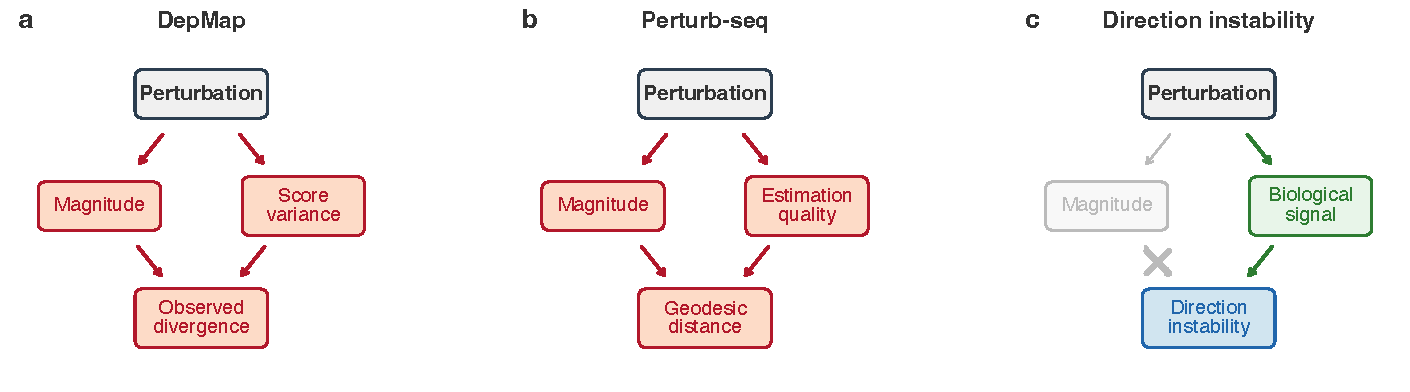
\includegraphics[width=\linewidth]{figures/fig6_causal_dag.pdf}
\caption{%
\textbf{Cross-domain confound structures.}
In all three domains, magnitude confounds operate through different
mechanisms, but cosine normalization renders direction instability
(right panel) invariant to perturbation magnitude. \textbf{Left:}~DepMap variance-based
scores conflate essentiality label with score variance.
\textbf{Center:}~Perturb-seq estimation-based metrics conflate
essentiality status with estimation quality.
\textbf{Right:}~Cosine normalization renders direction instability
invariant to perturbation magnitude, so the observed association
reflects biological signal.
Despite different confound mechanisms across domains, the validity
corrections produce the same qualitative result: population rankings
are preserved ($\rho > 0.83$) while item-level shifts identify
specific confound-dominated perturbations.}
\label{fig:cross_domain}
\end{figure}

The same geometric object---angular deviation of perturbation-response
directions across contexts---captures mechanism conservation in three
unrelated domains (Table~\ref{tab:cross_domain}). All three exhibit the
same pattern: the relevant validity condition preserves the global ranking
while identifying individual perturbations whose scores are most
confound-dominated.

\begin{table}[t]
\centering
\caption{Cross-domain summary. All three domains exceed the ``doesn't
bite'' threshold ($\rho \geq 0.83$). The LINCS HDAC gradient $\rho$
measures fine-grained ordering within a single drug class (6 compounds
in the selectivity gradient, Figure~\ref{fig:hdac});
the global 8{,}949-drug $\rho > 0.99$. H5 (transport stability) tests
predictive validity rather than rank preservation; the 66-fold
leave-one-out result (Table~\ref{tab:scorecard}) provides the strongest
domain-specific evidence for LINCS.}
\label{tab:cross_domain}
\small
\begin{tabular}{llrl}
\toprule
Domain & Correction & $N$ & $\rho$ \\
\midrule
LINCS (HDAC gradient) & Toxicity genes & 6 & 0.83 \\
LINCS (global) & Toxicity genes & 8{,}949 & $>$0.99 \\
Perturb-seq & Essential-gene subspace & 1{,}676 & 0.91 \\
JUMP-CP & Cell-health features & 25{,}254 & 0.99 \\
\bottomrule
\end{tabular}
\end{table}

The domain-specific failure modes differ: in drugs, cytotoxicity
produces high-instability signatures; in genetics, universal-essential
knockdowns produce high-distance subspaces (divergent lethal programs);
in morphology, cell-health features contribute a small fraction of
cross-source variance. All three invert the naive prediction that
``violence mimics transport.''

\subsection{Generalizability of the construct-validity procedure}

The validity ladder was tested on one geometric perturbation score
(direction instability) across three biological domains. The
\emph{procedure}---define interpretive threats, specify corrections
that target each threat, pre-register predictions about whether
corrections reorganize rankings, test empirically---applies to other
geometric scores that measure perturbation-response consistency, such as
connectivity scores \citep{subramanian2017next}, morphological similarity
indices, and Grassmannian distance metrics. What would change are the
domain-specific rungs: a connectivity score would require different
confound corrections than direction instability, but the same
structure of threat identification, correction, and pre-registered
testing applies. The effect size for phenotype projection ($\rho = 0.38$,
explaining ${\sim}14\%$ of variance) is moderate; contextualizing this
against other drug-mechanism prediction methods would help
practitioners judge whether this rung's evidence is sufficient for
their decisions.

\subsection{Scope and limitations}

Direction instability measures angular consistency of perturbation signatures
across contexts. It does not measure therapeutic efficacy, in-vivo
translatability, or clinical specificity. The validity ladder is a
construct-validation framework for interpretive warrant, not a surrogate
endpoint.

The drug experiments H3--H5 depend on shRNA knockdown signatures as
ground-truth on-target directions. shRNA has well-documented off-target
effects, which add noise to the ground truth. A CRISPRi
convergent-validity check did not
independently confirm the phenotype-projection result ($\rho = -0.12$,
$p = 0.16$, $n = 131$); the matched 114-drug comparison (shRNA
$\rho = 0.42$ vs.\ CRISPRi $\rho = -0.14$) points to the
pre-registered K562-only confound (CRISPRi signatures from a single
cell type are poor on-target directions for drugs acting in
non-hematopoietic contexts). The shRNA H3 result is not refuted but
neither is it reinforced. Drugs with unannotated targets
(7{,}398 of 8{,}949) are excluded from H3 and H4, limiting these rungs
to 17\% of the dataset. LINCS measures 978 landmark genes, restricting
the toxicity gene set to the landmark panel.

The Perturb-seq analysis uses $K = 2$ cell types, providing no Fr\'echet
variance, holonomy, or transport stability test. Both screens target
DepMap-essential genes, so the HP3 ``non-essential'' group consists of
sub-threshold essentials rather than genuinely non-essential genes. A
genome-wide screen with genuine non-essential controls would be sharper,
though the label-permutation null rules out the library-overlap confound.

The transport-stable bracket formula (Eq.~\ref{eq:ts}) is a heuristic
linear combination of direction instability and Fr\'echet variance, not a
principled geometric operation on the signature manifold. The penalty
weight $\lambda$ was inherited from the companion paper
\citep{tower2026drug} and was not optimized for this evaluation. A
sensitivity analysis across a range of $\lambda$ values would strengthen
the claim that the H5 advantage is robust to the specific penalty
weight; we report this specific formula because it was pre-registered,
and post-hoc $\lambda$ optimization would compromise the pre-registration.
A ratio or a geodesic-based combination might perform differently.

The validity ladder draws an analogy to Bradford Hill criteria for causal
inference. Bradford Hill criteria are individually neither necessary nor
sufficient for establishing causation; they are heuristic guidelines. The
validity ladder shares this character: it is a structured set of proof
obligations rather than a formal deductive system. Each rung eliminates
a specific threat, but satisfying all tested rungs does not
\emph{guarantee} that a mechanistic claim is correct---it guarantees
that specific alternatives have been ruled out.

JUMP-CP cell-health features were defined by substring matching rather
than by correlation with an independent viability assay. The 78\% attrition
from the full dataset biases the retained set toward well-replicated
compounds.

\section{Conclusions}

We have proposed and tested a construct-validity framework for geometric
perturbation scores, using direction instability as a case study across
three biological domains (drug transcriptomics, genetic perturbation
subspaces, morphological profiles). Validity conditions do not improve the
score's ability to rank perturbations---the ranking is already biologically
meaningful in all three domains ($\rho > 0.99$ for LINCS, $0.91$ for
Perturb-seq, $0.99$ for JUMP-CP after correction). They improve the
practitioner's ability to make claims about that ranking and to make
decisions based on those claims.

The procedure tested here---threat identification, correction
specification, pre-registered prediction, empirical test---is applicable
to any geometric score measuring perturbation-response consistency across
contexts. Phenotype projection separates on-target from off-target
consistency ($\rho = 0.38$ vs.\ $-0.04$); variance correction
outpredicts the raw score in all 66 leave-one-out folds
($p_{\text{Wilcoxon}} = 8.2 \times 10^{-13}$, mean
$\Delta\rho = +1.10$); localization helps for intracellular enzyme
targets but not receptor-mediated drugs, constraining where specific
rungs apply. The domain-specific failure modes differ, but the pattern
is the same: correction preserves population rankings while identifying
individual perturbations most susceptible to confounding. The validity
ladder provides a structured procedure for accumulating evidence that
a geometric perturbation score licenses mechanistic inference.

\section*{Declarations}

\subsection*{Ethics approval and consent to participate}
Not applicable. This study uses only publicly available datasets
(LINCS L1000, Perturb-seq, JUMP-CP, DepMap) with no human subjects
research.

\subsection*{Consent for publication}
Not applicable.

\subsection*{Availability of data and materials}
All data used in this study are publicly available: LINCS L1000
(GEO GSE92742), Perturb-seq \citep{replogle2022mapping}, JUMP-CP
\citep{chandrasekaran2023jump}, DepMap \citep{dempster2021chronos}.
Code, pre-registration commits (SHA \texttt{8d74bd0} for initial
freeze; SHA \texttt{f3c88ed}, tag \texttt{prereg-extended-psb}, for
extended pre-registration), deviation log, and all experimental
scripts are available at
\url{https://github.com/elliottower/direction-instability-drug-validity}.
The repository was public before the pre-registration freeze.

\subsection*{Competing interests}
The author declares no competing interests.

\subsection*{Funding}
This work received no external funding.

\subsection*{Authors' contributions}
ET conceived the study, designed the validity framework, conducted
all experiments, and wrote the manuscript.

\subsection*{Use of AI-assisted technologies}
Claude (Anthropic) was used as a writing and analysis assistant during manuscript preparation. The author directed all analytical decisions, verified all numerical results against source data, and takes full responsibility for the content. The validity framework, pre-registered hypotheses, all experimental results, and interpretations are the author's own. No AI tool is listed as an author.

\subsection*{Acknowledgements}
Not applicable.

\subsection*{Authors' information}
ET is an independent researcher focused on construct validity
and geometric methods for perturbation biology.

\subsection*{Companion papers}
Direction instability and the transport-stable bracket formula are
defined and validated in a companion paper on LINCS L1000 drug
transport (submitted to PLOS Computational Biology,
PCOMPBIOL-S-26-02155; \citep{tower2026drug}). The cross-domain
direction-instability atlas (LINCS, Perturb-seq, JUMP-CP) is
described in a companion paper submitted to GigaScience
(GIGA-D-26-00229; \citep{tower2026atlas}). Both are available as
Zenodo preprints. The present paper tests construct-validity
conditions on top of these prior results.

\bibliographystyle{unsrtnat}
\bibliography{references}

\end{document}
